\usepackage{booktabs}

\begin{frame}
    \frametitle{Spectrum of p2o Map}
    \begin{figure}
        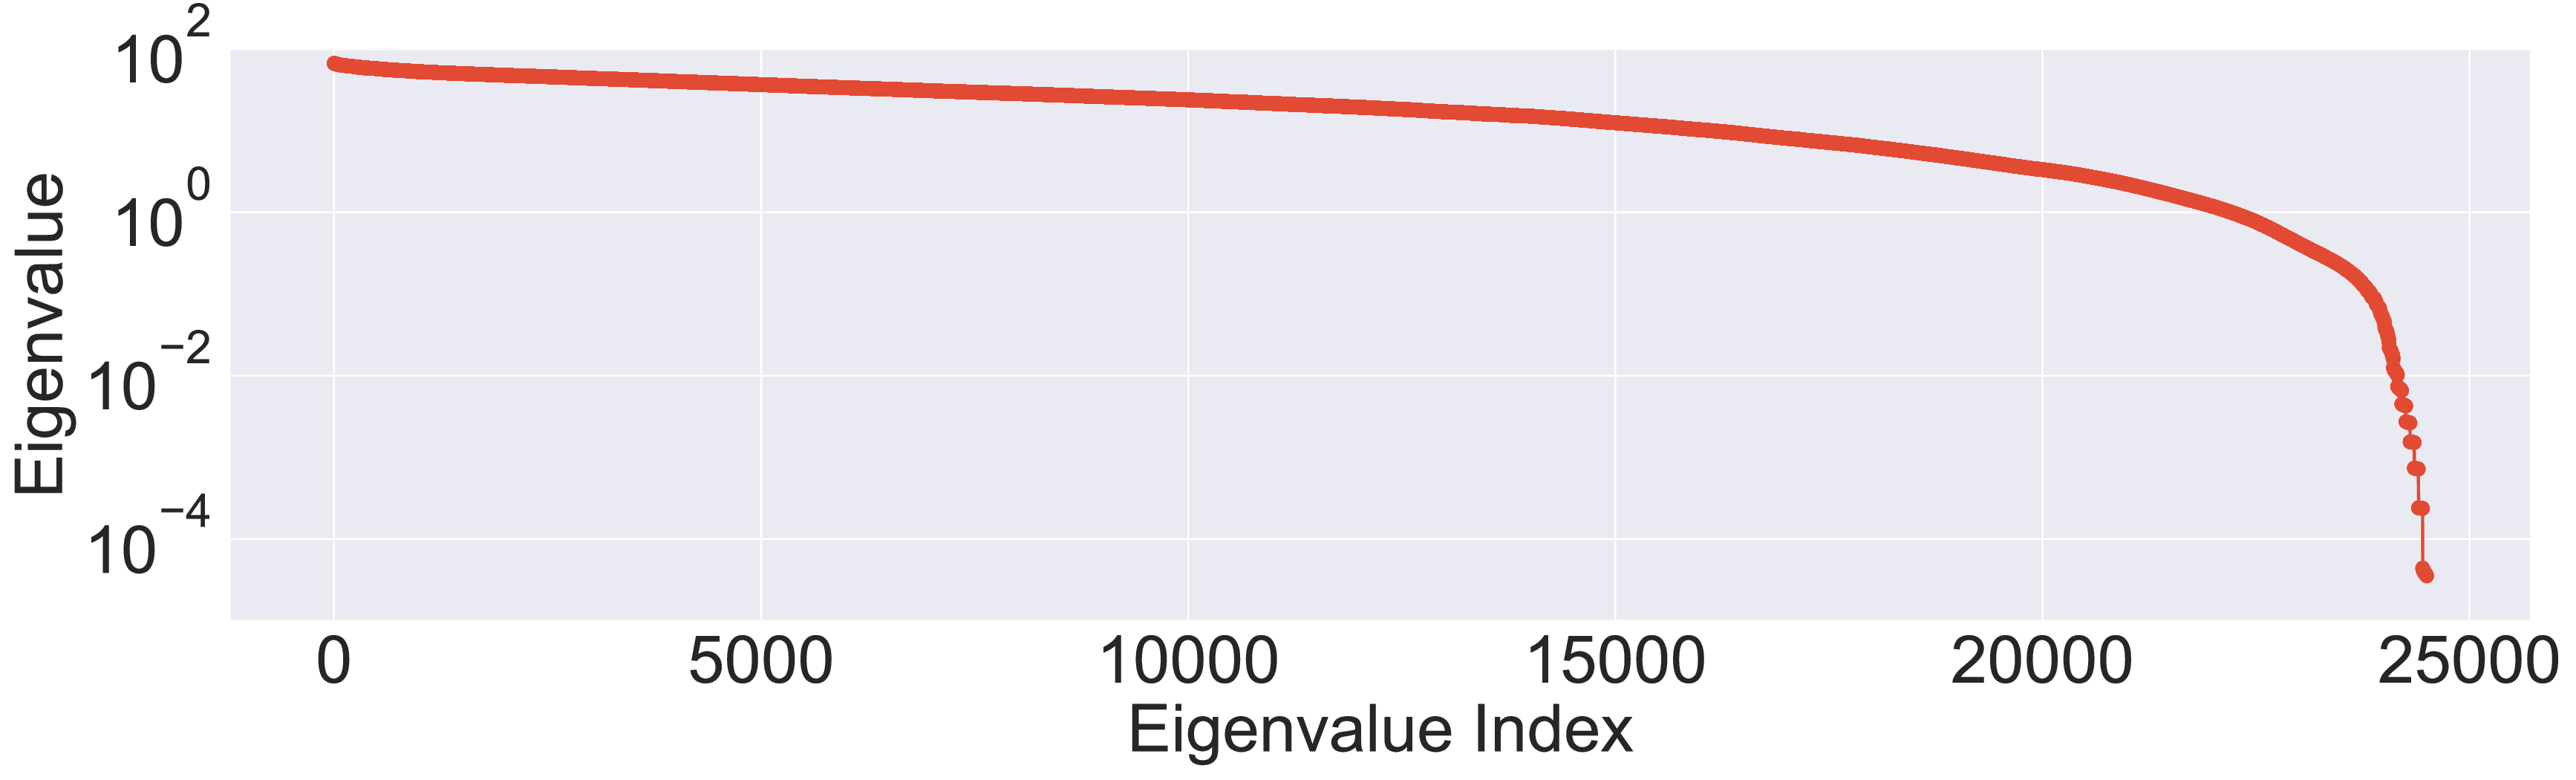
\includegraphics[width=\textwidth]{JMM/images/prior_spectra/evals_p2o.png}
        \caption{Eigenvalues of \(\mathbf{F} \mathbf{F}^*\) for the test configuration}
    \end{figure}
    \begin{itemize}
        \item Spectral decay of \(\mathbf{K}\) is not fast enough to use low-rank approximations
    \end{itemize}
\end{frame}

\begin{frame}
    \frametitle{Time and Memory Report}
    \begin{table}
        \toprule
        \textbf{Phase} & \textbf{Compute Time} & \textbf{Memory/Storage} \\
        \midrule
        Phase 1: 49 adjoint PDE solves & 49 \(\times\) 8 min \newline ~6.5 hrs & 49 \(\times\) 1.053 GB \newline ~52 GB \\
        Phase 2: prior solves to form \(\mathbf{G}^*\) & 49 \(\times\) 84 ms \newline ~4.12 s & 49 \(\times\) 1.053 GB \newline ~52 GB \\
        Phase 2: compute and store \(\mathbf{K}\) & 24,500 \(\times\) 22 ms \newline ~10 min & 24,500\(^2\) \(\times\) 8 b \newline ~4.8 GB \\
        Factorize \(\mathbf{K}\) & 1.18 s & stored over \(\mathbf{K}\) \\
        \textbf{Phase 3: compute \(\mathbf{m}_{\text{map}}\)} & 57 ms & \(\mathbf{m}_{\text{map}}\): 1.053 GB \\
        \textbf{Phase 3: compute QoI} & 3 ms & \(\mathbf{q}\): negligible \\
        \bottomrule
    \end{table}
    \caption{Time and memory report for each phase of the inversion. Phase 1 run on 32 SPR nodes of \href{https://docs.tacc.utexas.edu/hpc/stampede3/}{Stampede3}. Phases 2 and 3 run on 8 nodes of \href{https://docs.tacc.utexas.edu/hpc/lonestar6/}{Lonestar6} (24 A100 GPUs)}
\end{frame}

\begin{frame}
    \frametitle{Online Compute Time}
    \begin{table}
        \toprule
        \textbf{Step} & \textbf{Compute Time} \\
        \midrule
        2 \(\mathbf{G}^*\) matvecs & 0.022s \\
        1 \(\mathbf{F}\) matvec & 0.011s \\
        1 \(\mathbf{F}_{\!\text{pred}}\) matvec & 0.003s \\
        1 \(\mathbf{K}\) solve & 0.024s \\
        \textbf{Total} & 0.06s \\
        \bottomrule
    \end{table}
    \begin{itemize}
        \item \textbf{~44,000x} speedup of p2o application vs. PDE solves on 32 SPR nodes of \href{https://docs.tacc.utexas.edu/hpc/stampede3/}{Stampede3}
        \item \textbf{~196,000x} speedup of p2o application vs. PDE solves on 32 CLX nodes of \href{https://docs.tacc.utexas.edu/hpc/frontera/}{Frontera}
    \end{itemize}
\end{frame}

\begin{frame}
    \frametitle{3D Inversion: True Parameter and Observations}
    \begin{figure}
        \centering
        \subfloat[\textbf{Left:} Synthetic parameter field (seafloor motion) composed of superimposed Gaussian deformations]{
            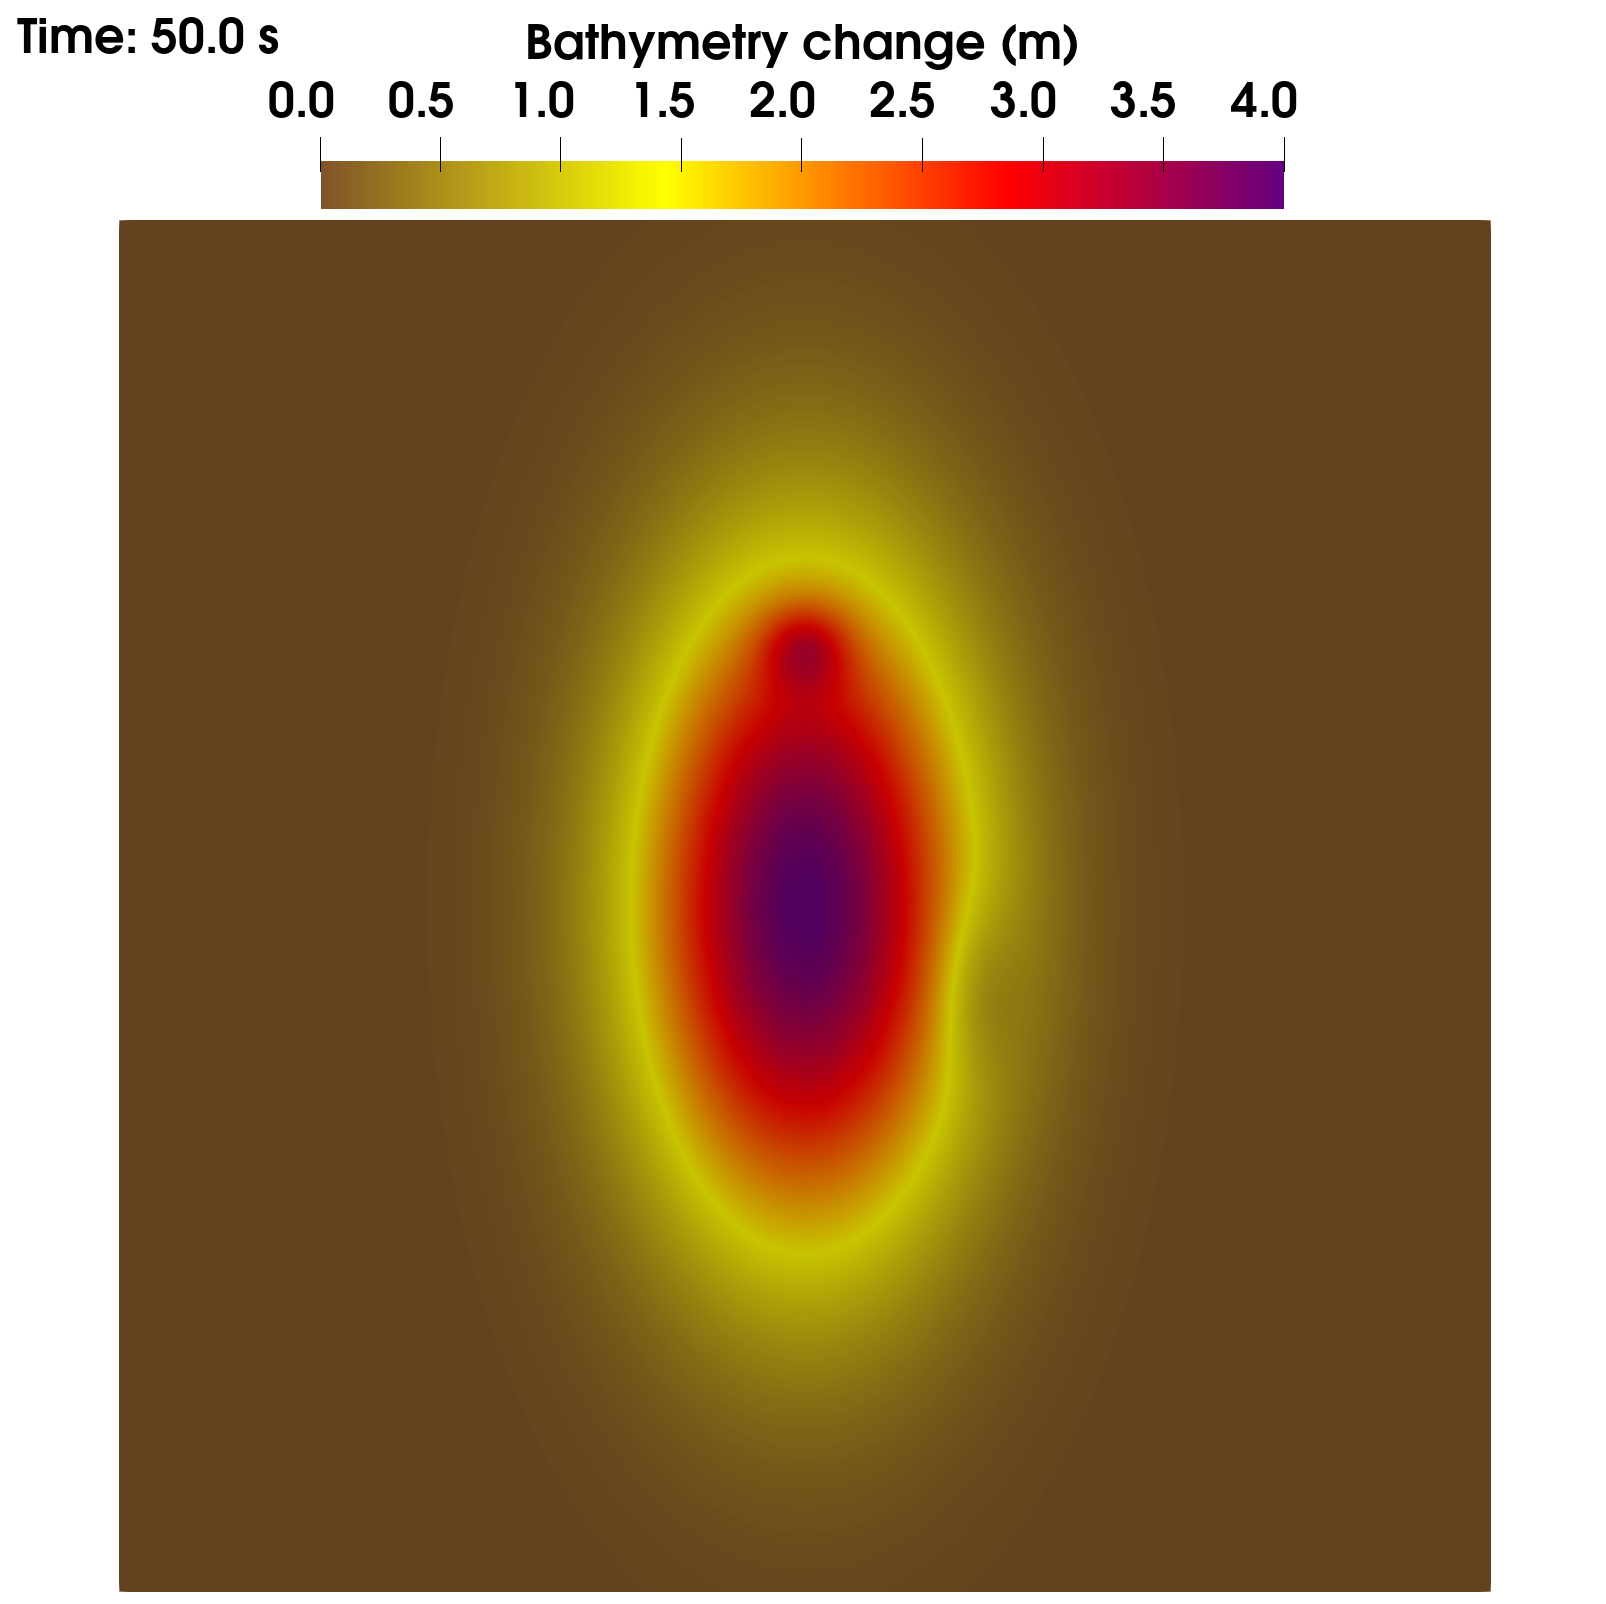
\includegraphics[width=0.45\textwidth]{JMM/images/results/bathymetry_true.gif}
        }
        \hfill
        \subfloat[\textbf{Right:} True seafloor pressure]{
            \includegraphics[width=0.45\textwidth]{JMM/images/results/true_pressure.gif}
        }
    \end{figure}
\end{frame}

\begin{frame}
    \frametitle{3D Inversion: Inverse Solution}
    \begin{figure}
        \centering
        \subfloat[\textbf{Left:} Synthetic observations with 6\% relative noise]{
            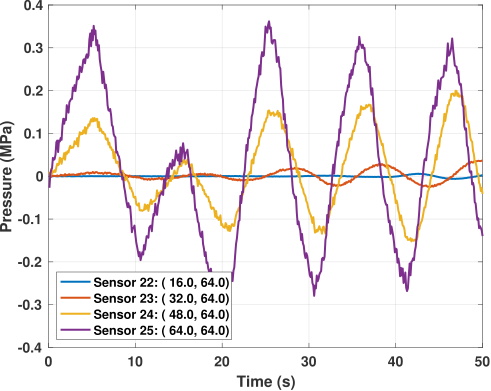
\includegraphics[width=0.45\textwidth]{JMM/images/results/noisy_3.svg}
        }
        \hfill
        \subfloat[\textbf{Right:} Relative error in the inferred mean seafloor velocity]{
            \begin{table}
                \toprule
                \textbf{Noise Level} & \textbf{Rel. Error} \\
                \midrule
                2\% & 0.077554 \\
                4\% & 0.083632 \\
                6\% & 0.094816 \\
                \bottomrule
            \end{table}
        }
    \end{figure}
\end{frame}

\begin{frame}
    \frametitle{3D Inversion: Inferred Parameter Field (Real-Time)}
    \begin{figure}
        \centering
        \subfloat[\textbf{Left:} True total seafloor displacement (time-integrated parameter field)]{
            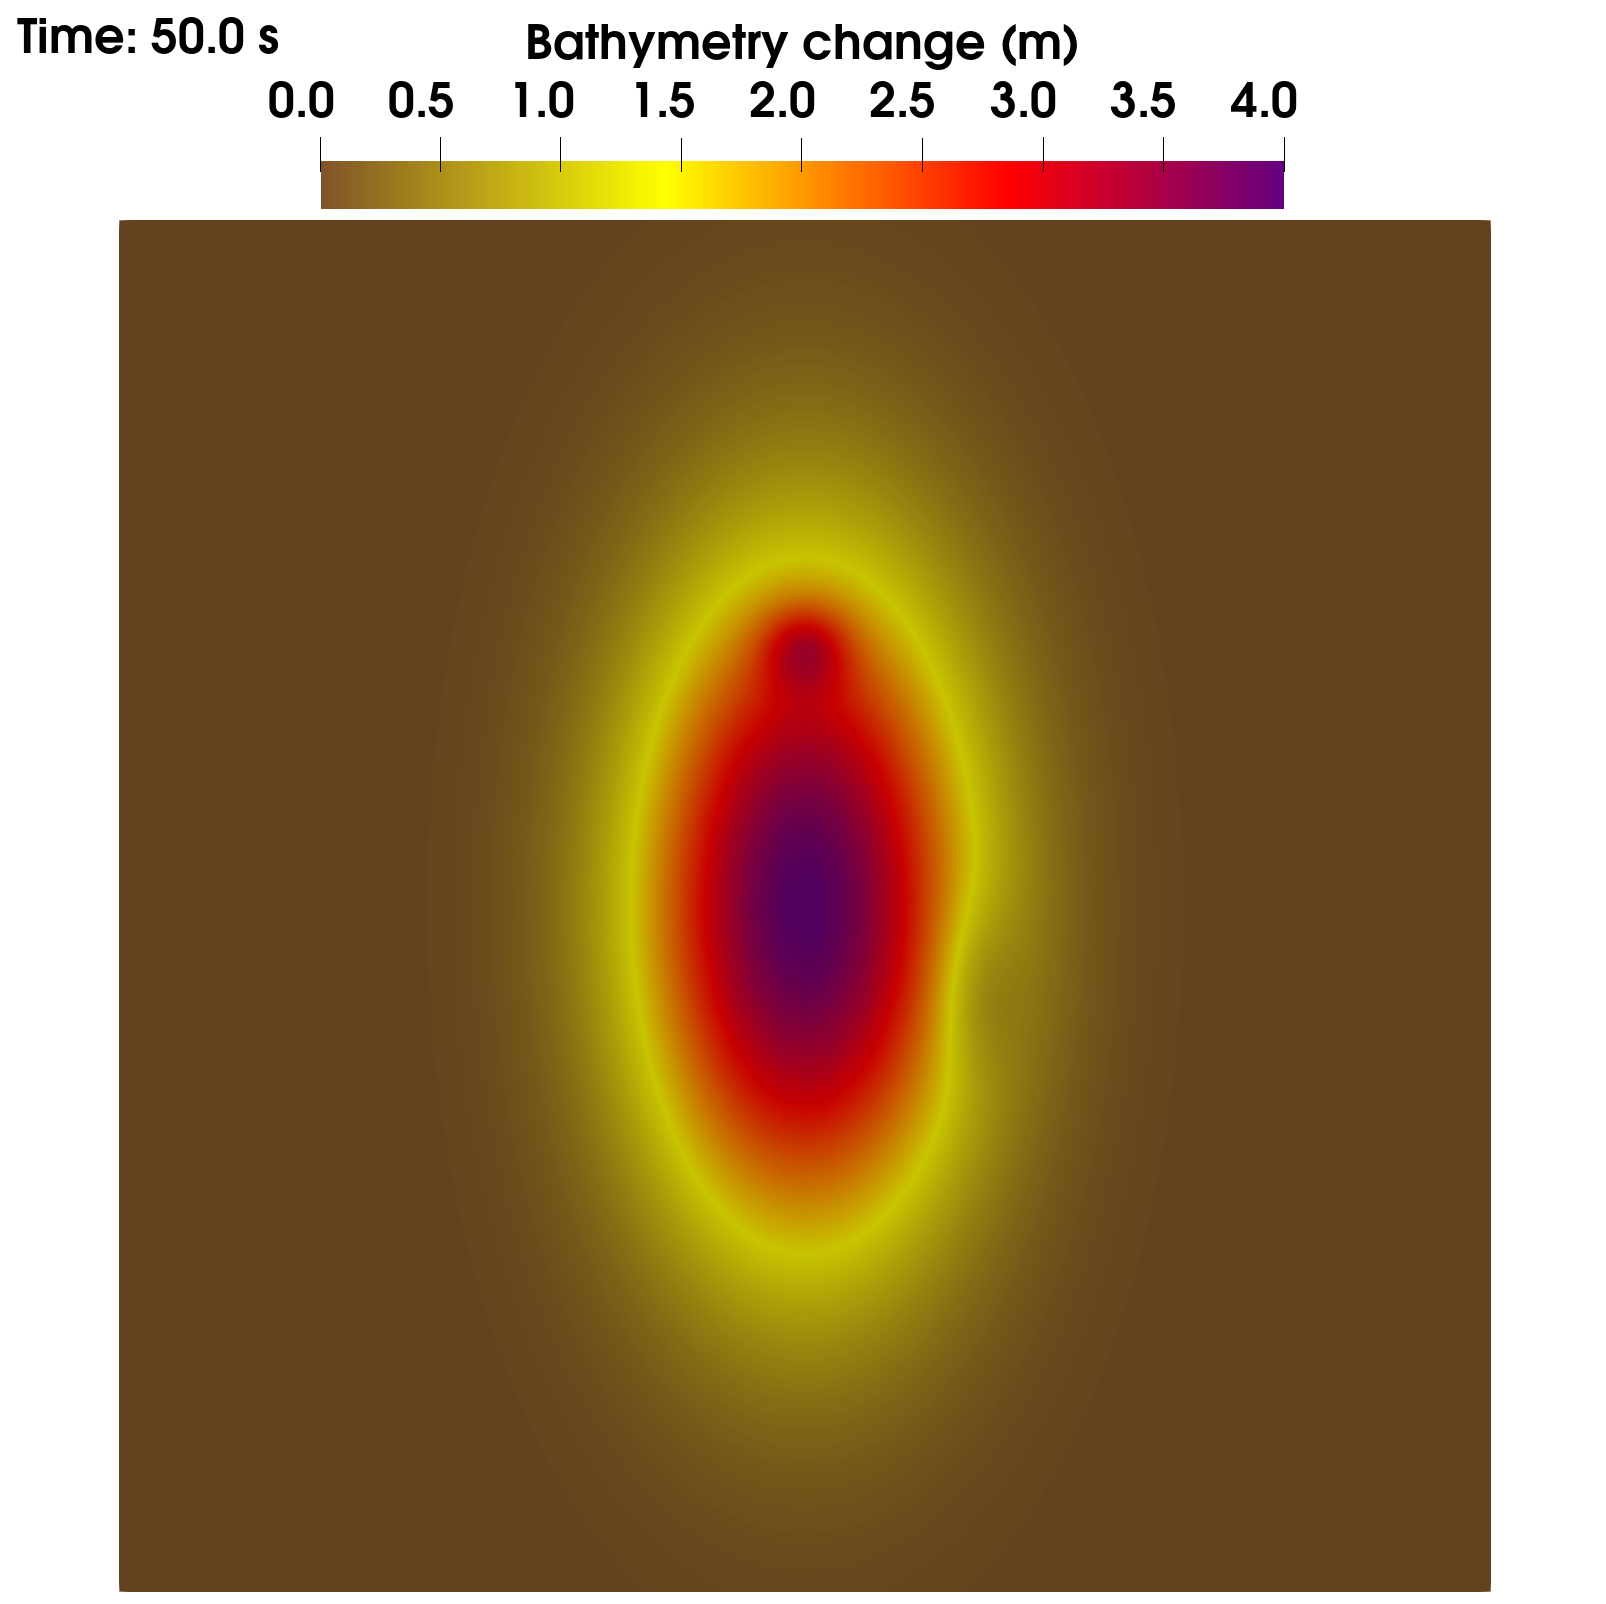
\includegraphics[width=0.3\textwidth]{JMM/images/results/bathymetry_true.png}
        }
        \hfill
        \subfloat[\textbf{Middle:} Total seafloor displacement inferred from synthetic observations with 6\% relative additive noise]{
            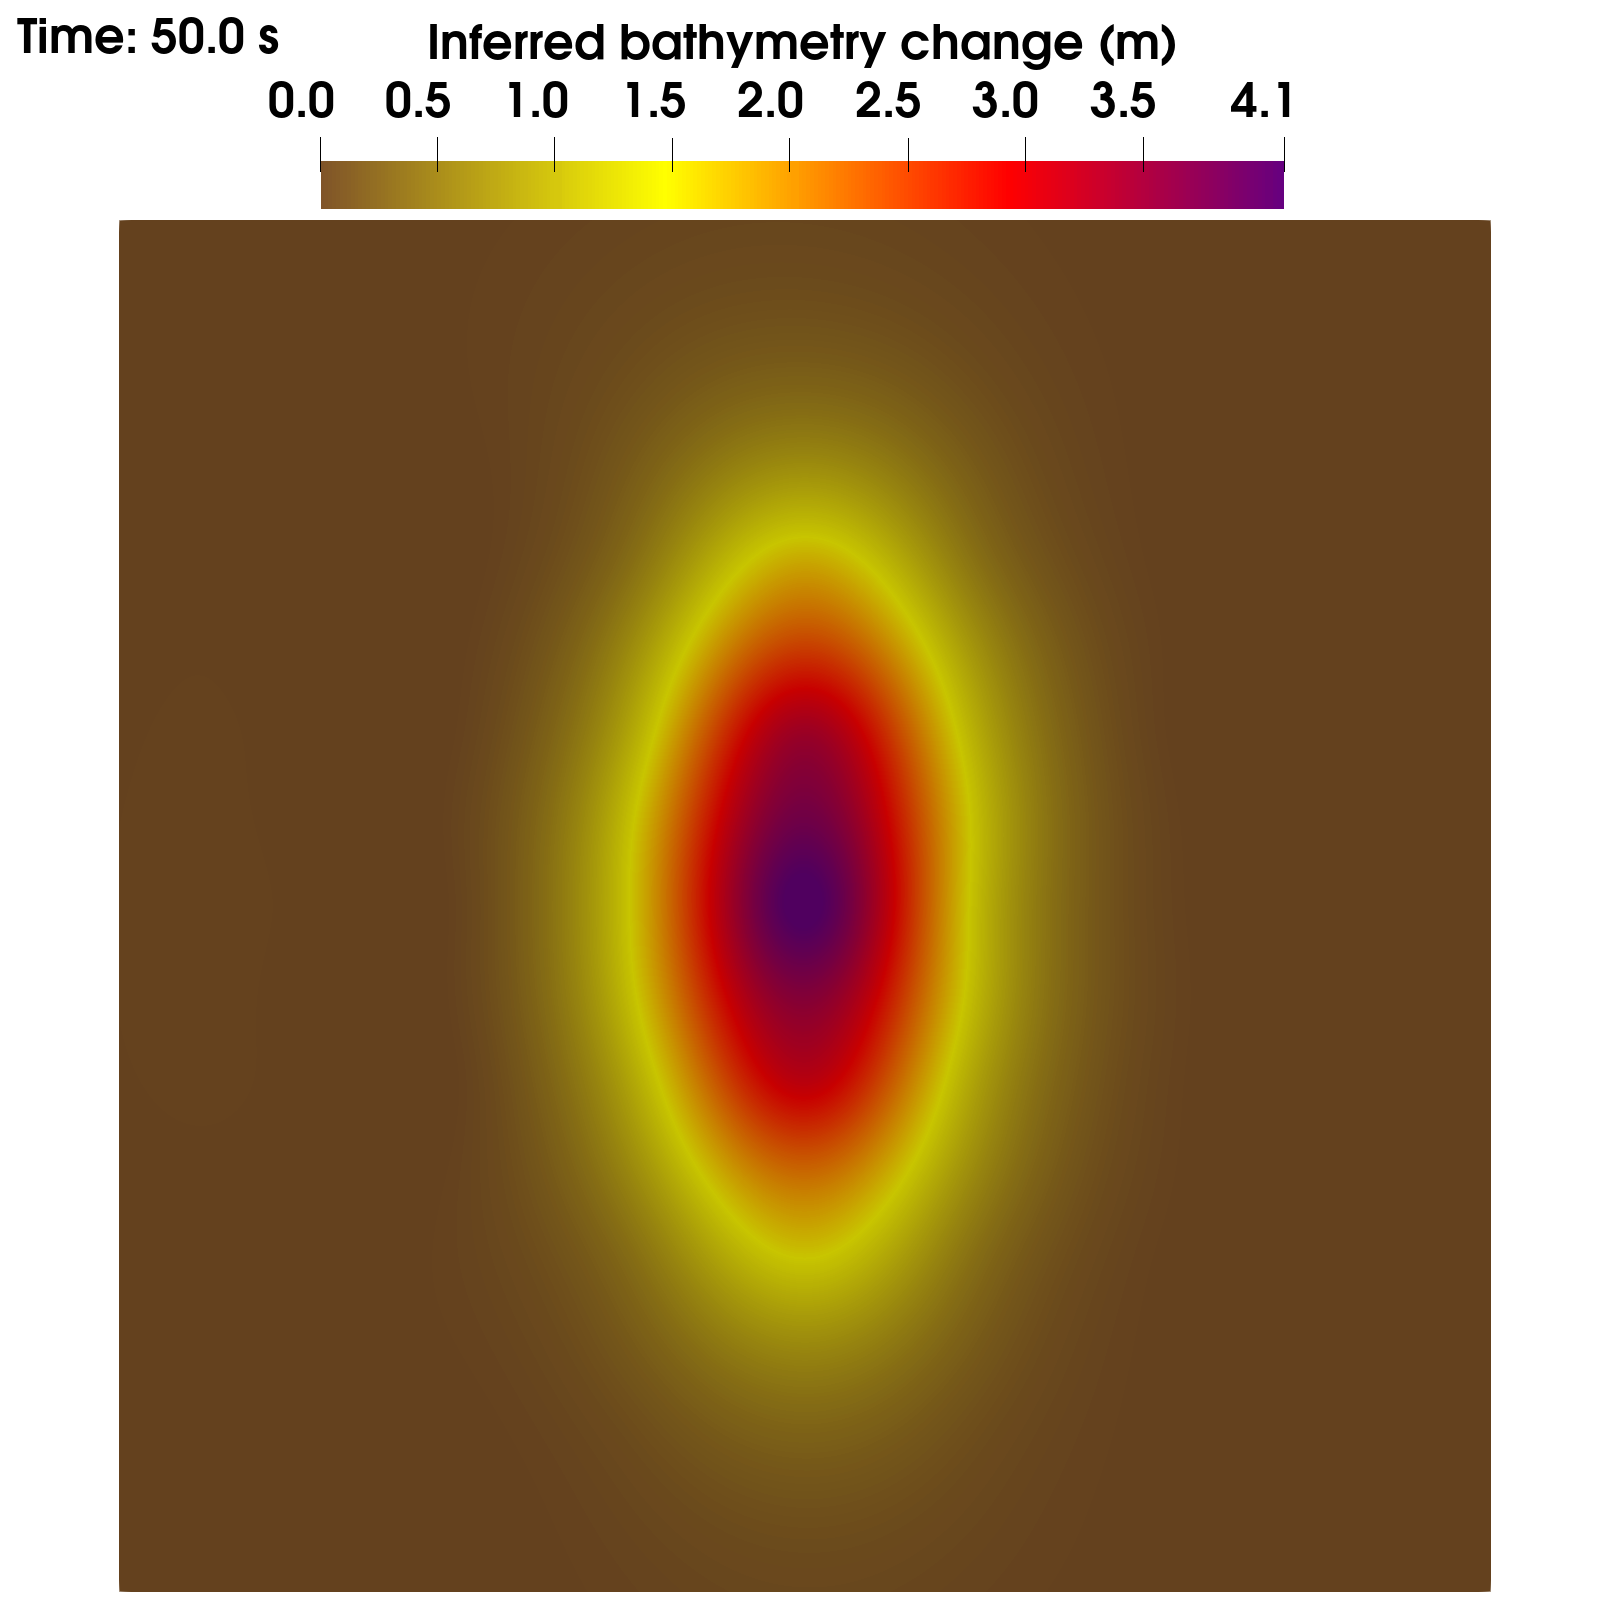
\includegraphics[width=0.3\textwidth]{JMM/images/results/bathymetry_inv.png}
        }
        \hfill
        \subfloat[\textbf{Right:} Difference between inferred and true total seafloor displacement]{
            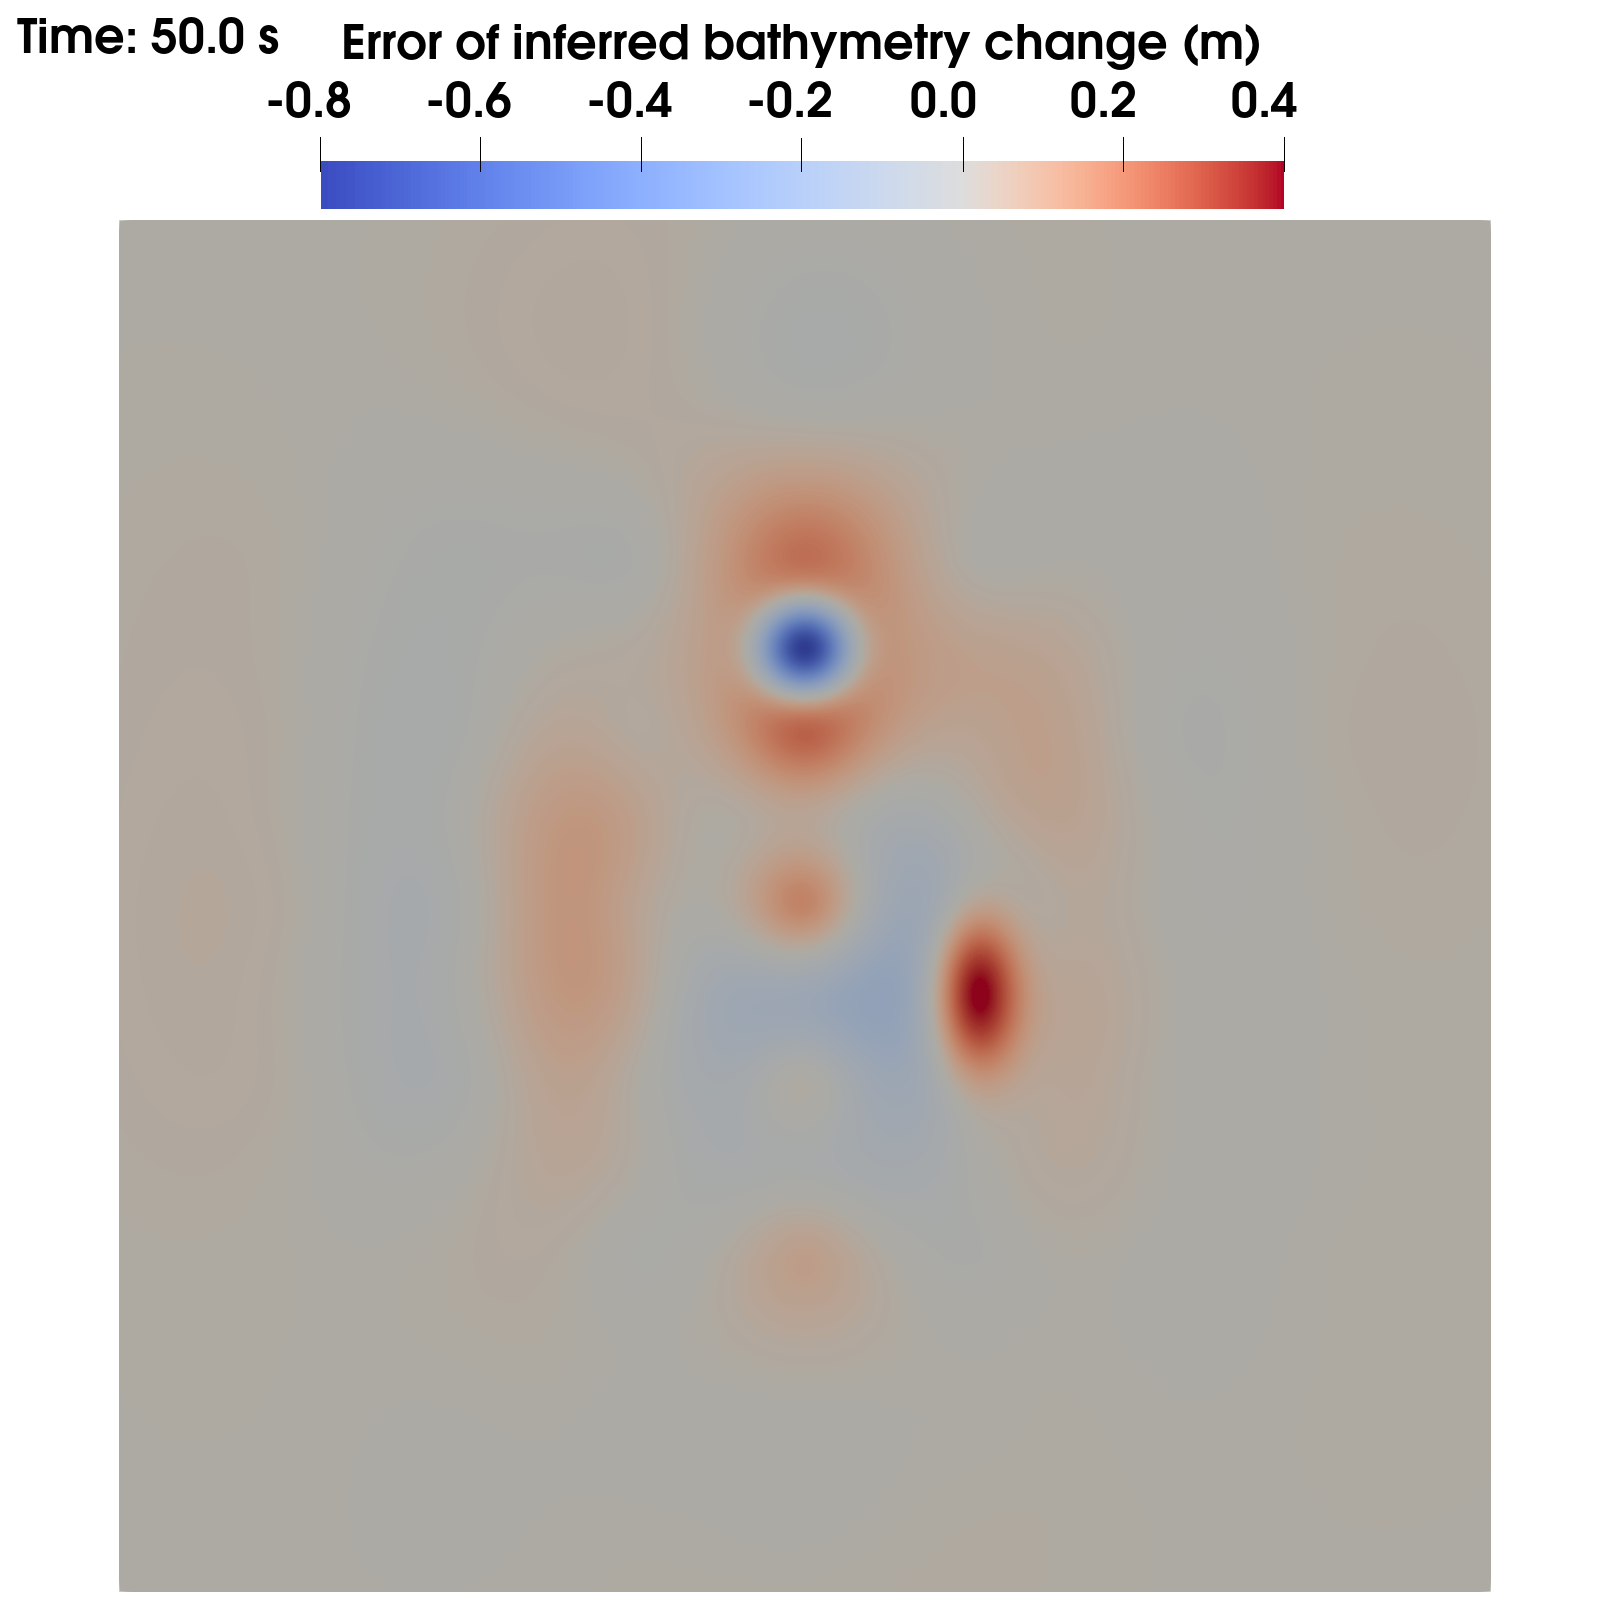
\includegraphics[width=0.3\textwidth]{JMM/images/results/bathymetry_diff.png}
        }
    \end{figure}
\end{frame}

\begin{frame}
    \frametitle{3D Inversion: Pressure Reconstruction}
    \begin{figure}
        \centering
        \subfloat[\textbf{Left:} Seafloor pressure field reconstructed with the parameter field inferred from synthetic observations with 6\% relative additive noise]{
            \includegraphics[width=0.45\textwidth]{JMM/images/results/inv_pressure.gif}
        }
        \hfill
        \subfloat[\textbf{Right:} Difference between reconstructed and true pressure field]{
            \includegraphics[width=0.45\textwidth]{JMM/images/results/diff_pressure.gif}
        }
    \end{figure}
\end{frame}

\begin{frame}
    \frametitle{3D Inversion: Surface-Gravity Wave}
    \begin{figure}
        \centering
        \subfloat[\textbf{Left:} Amplitude of surface gravity wave obtained from true parameter field]{
            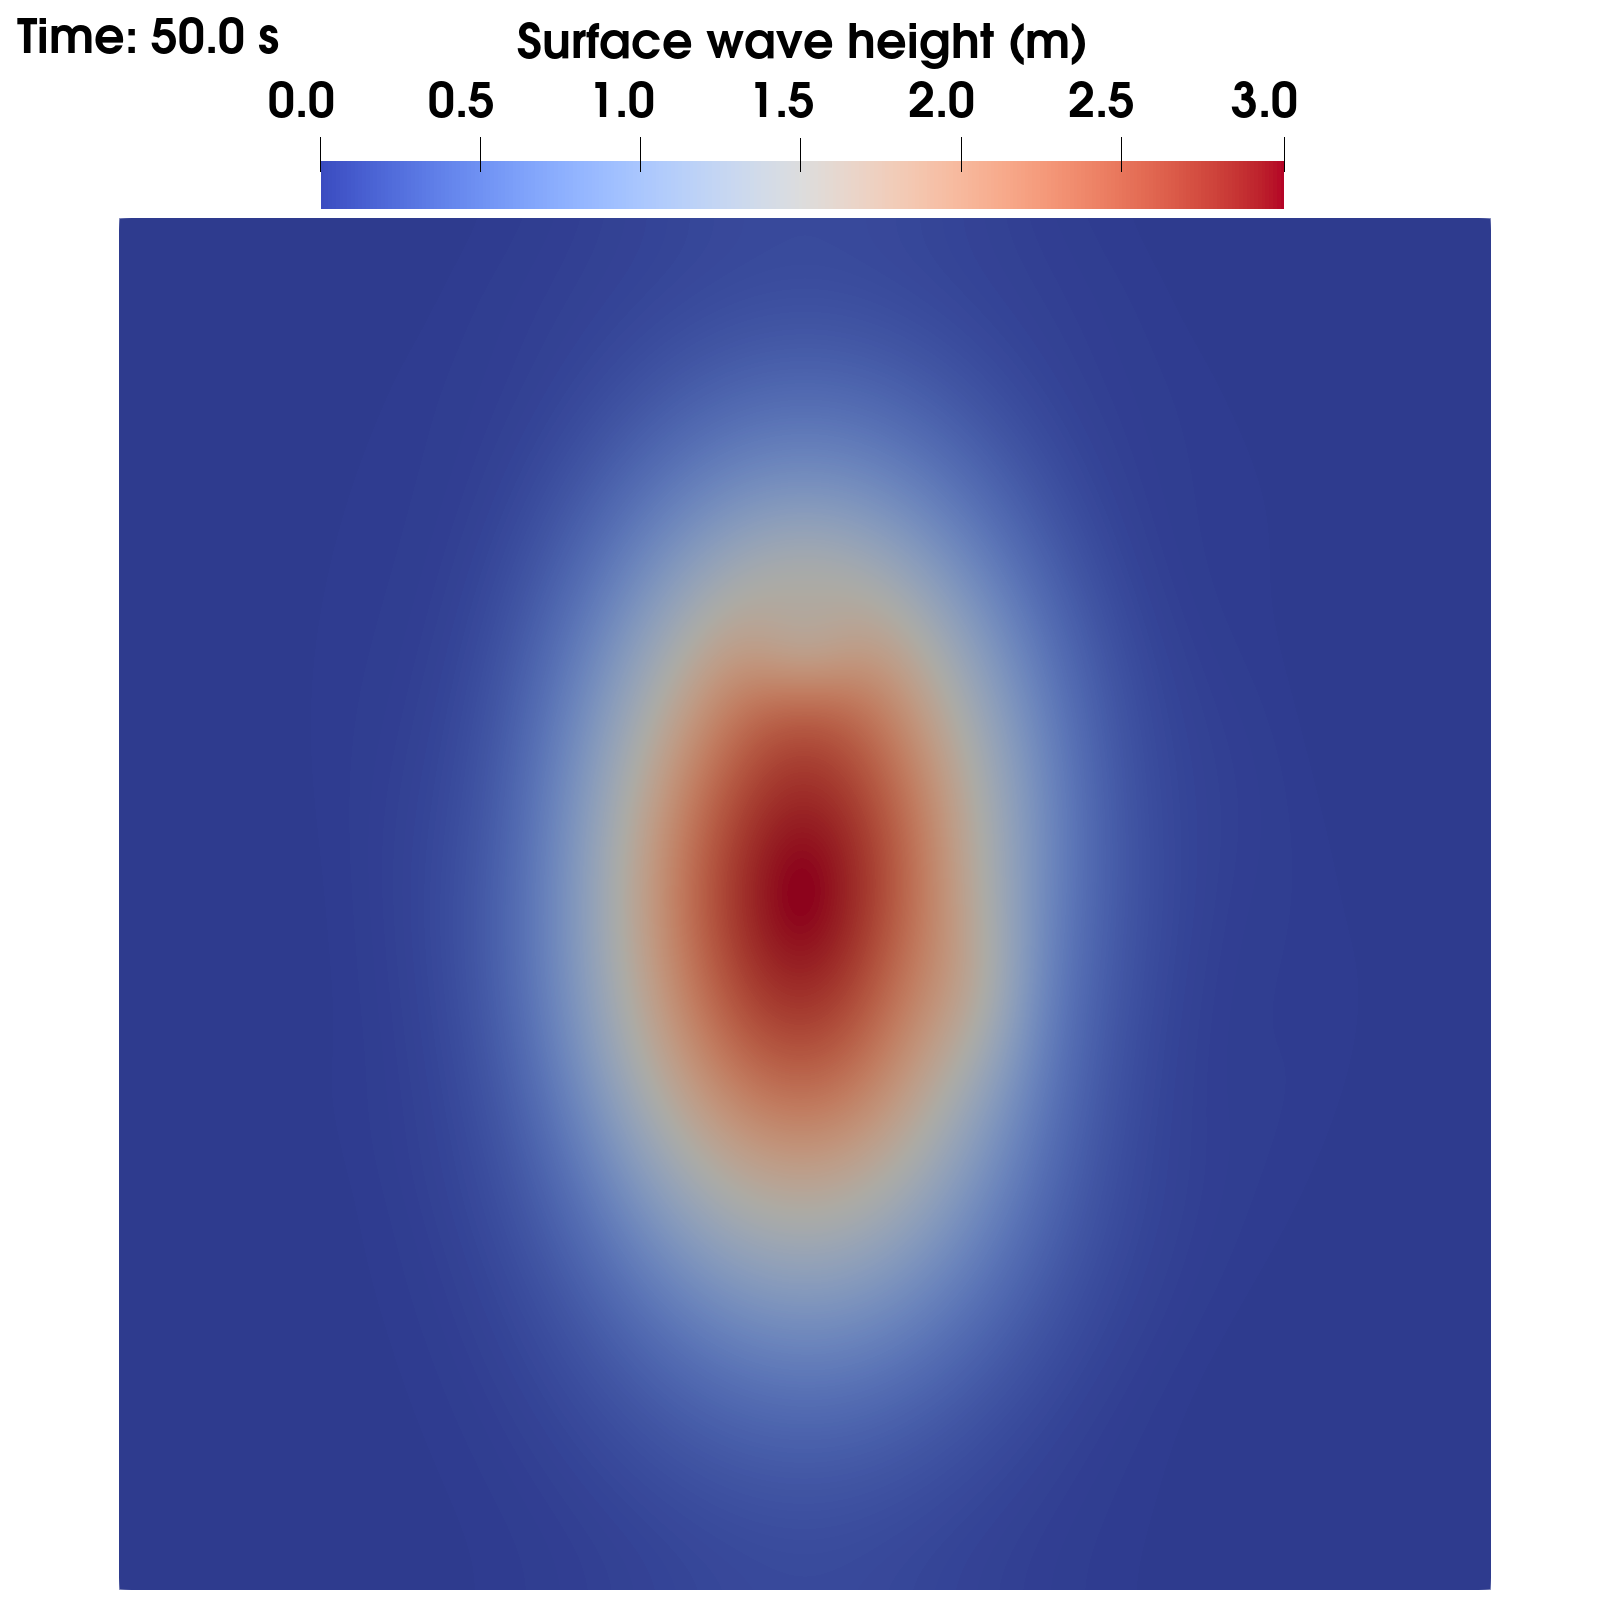
\includegraphics[width=0.3\textwidth]{JMM/images/results/wave_true.png}
        }
        \hfill
        \subfloat[\textbf{Middle:} Amplitude of surface gravity wave reconstructed with the parameter field inferred from synthetic observations with 6\% relative additive noise]{
            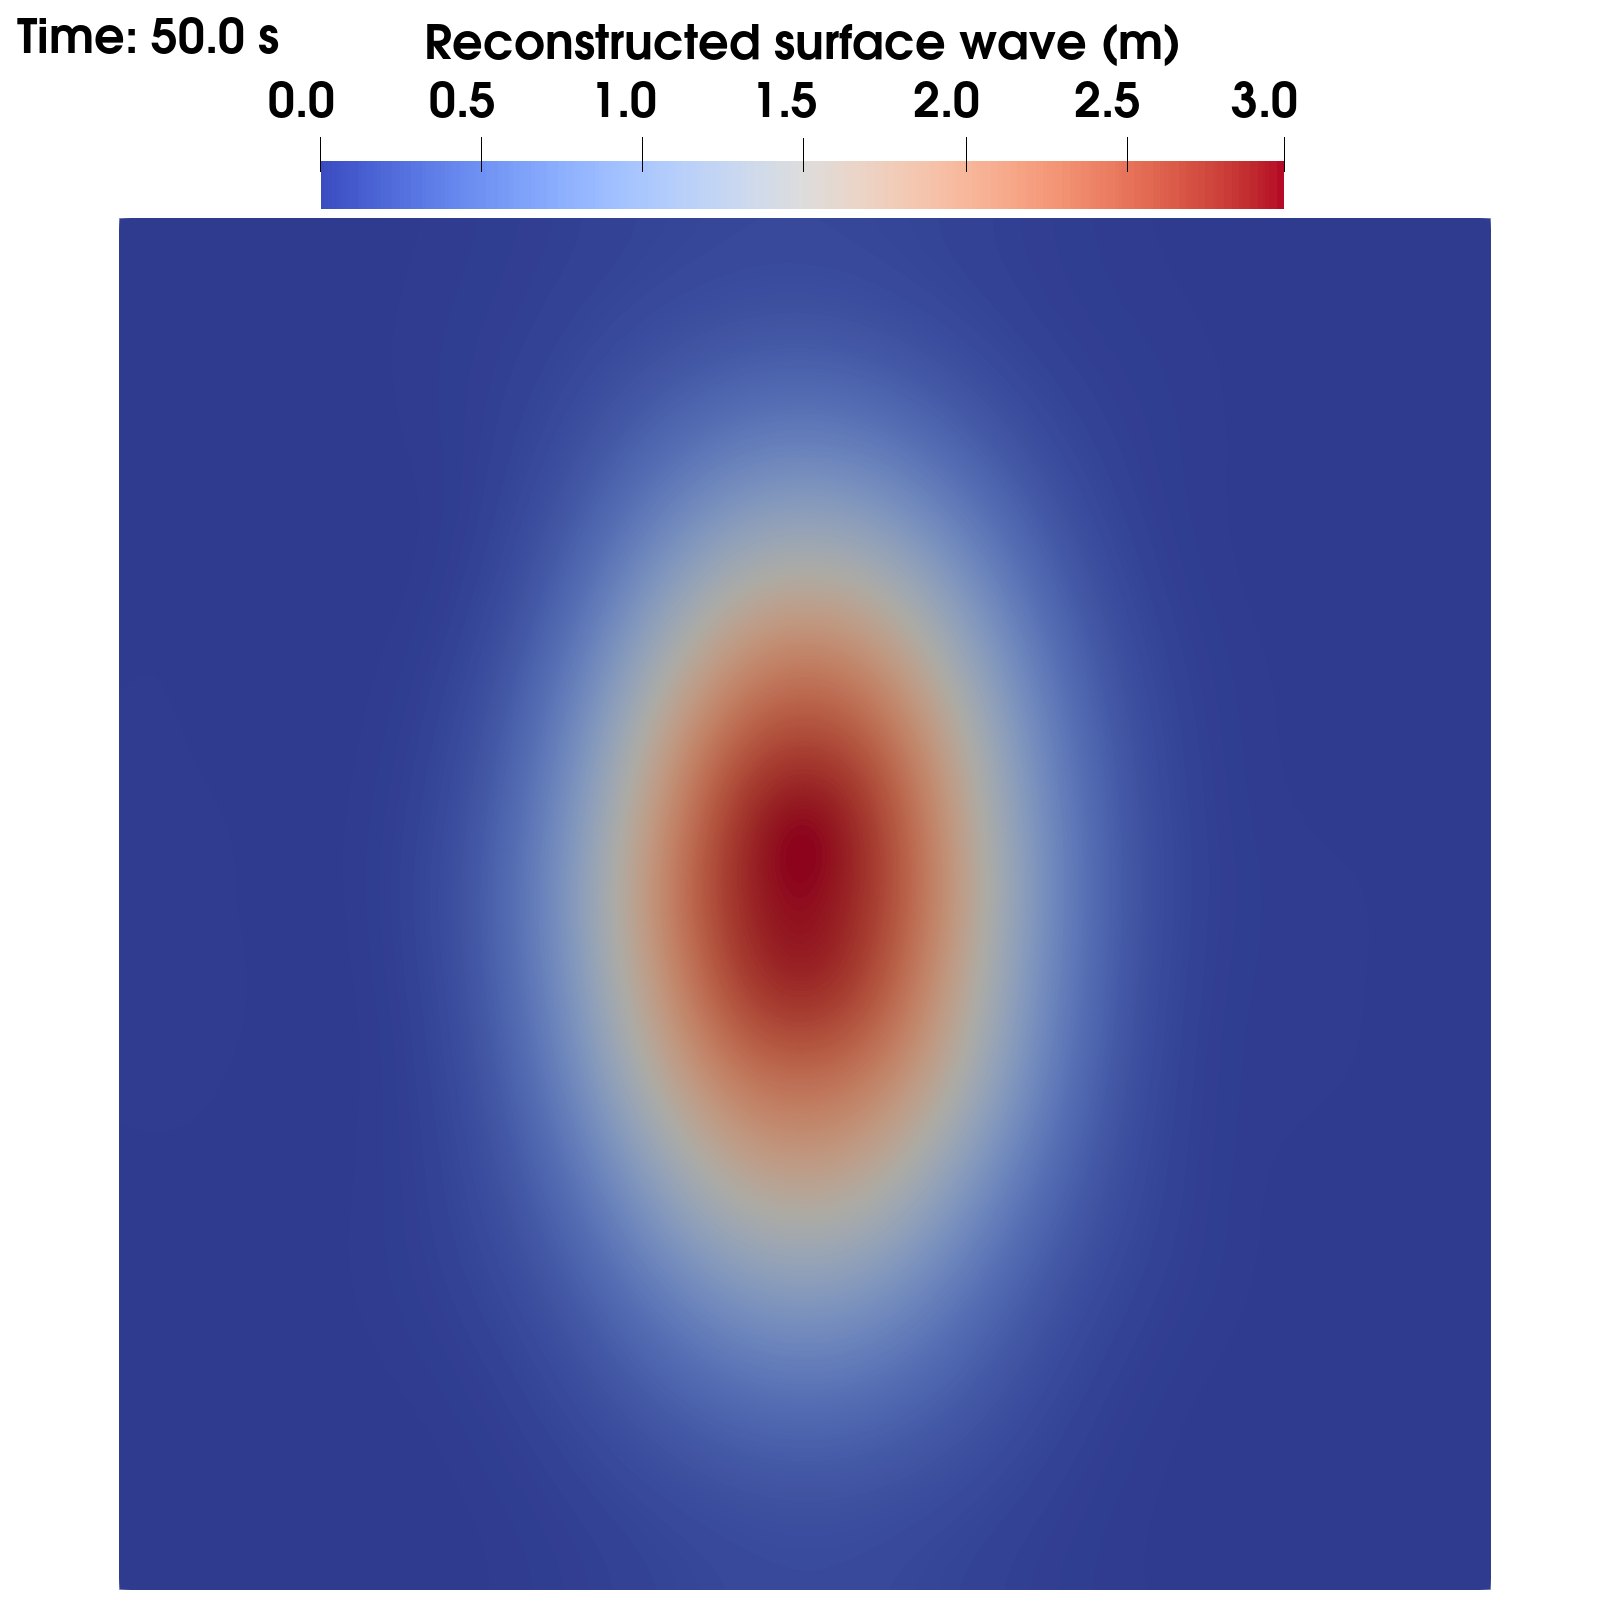
\includegraphics[width=0.3\textwidth]{JMM/images/results/wave_inv.png}
        }
        \hfill
        \subfloat[\textbf{Right:} Difference between reconstructed and true surface-gravity wave]{
            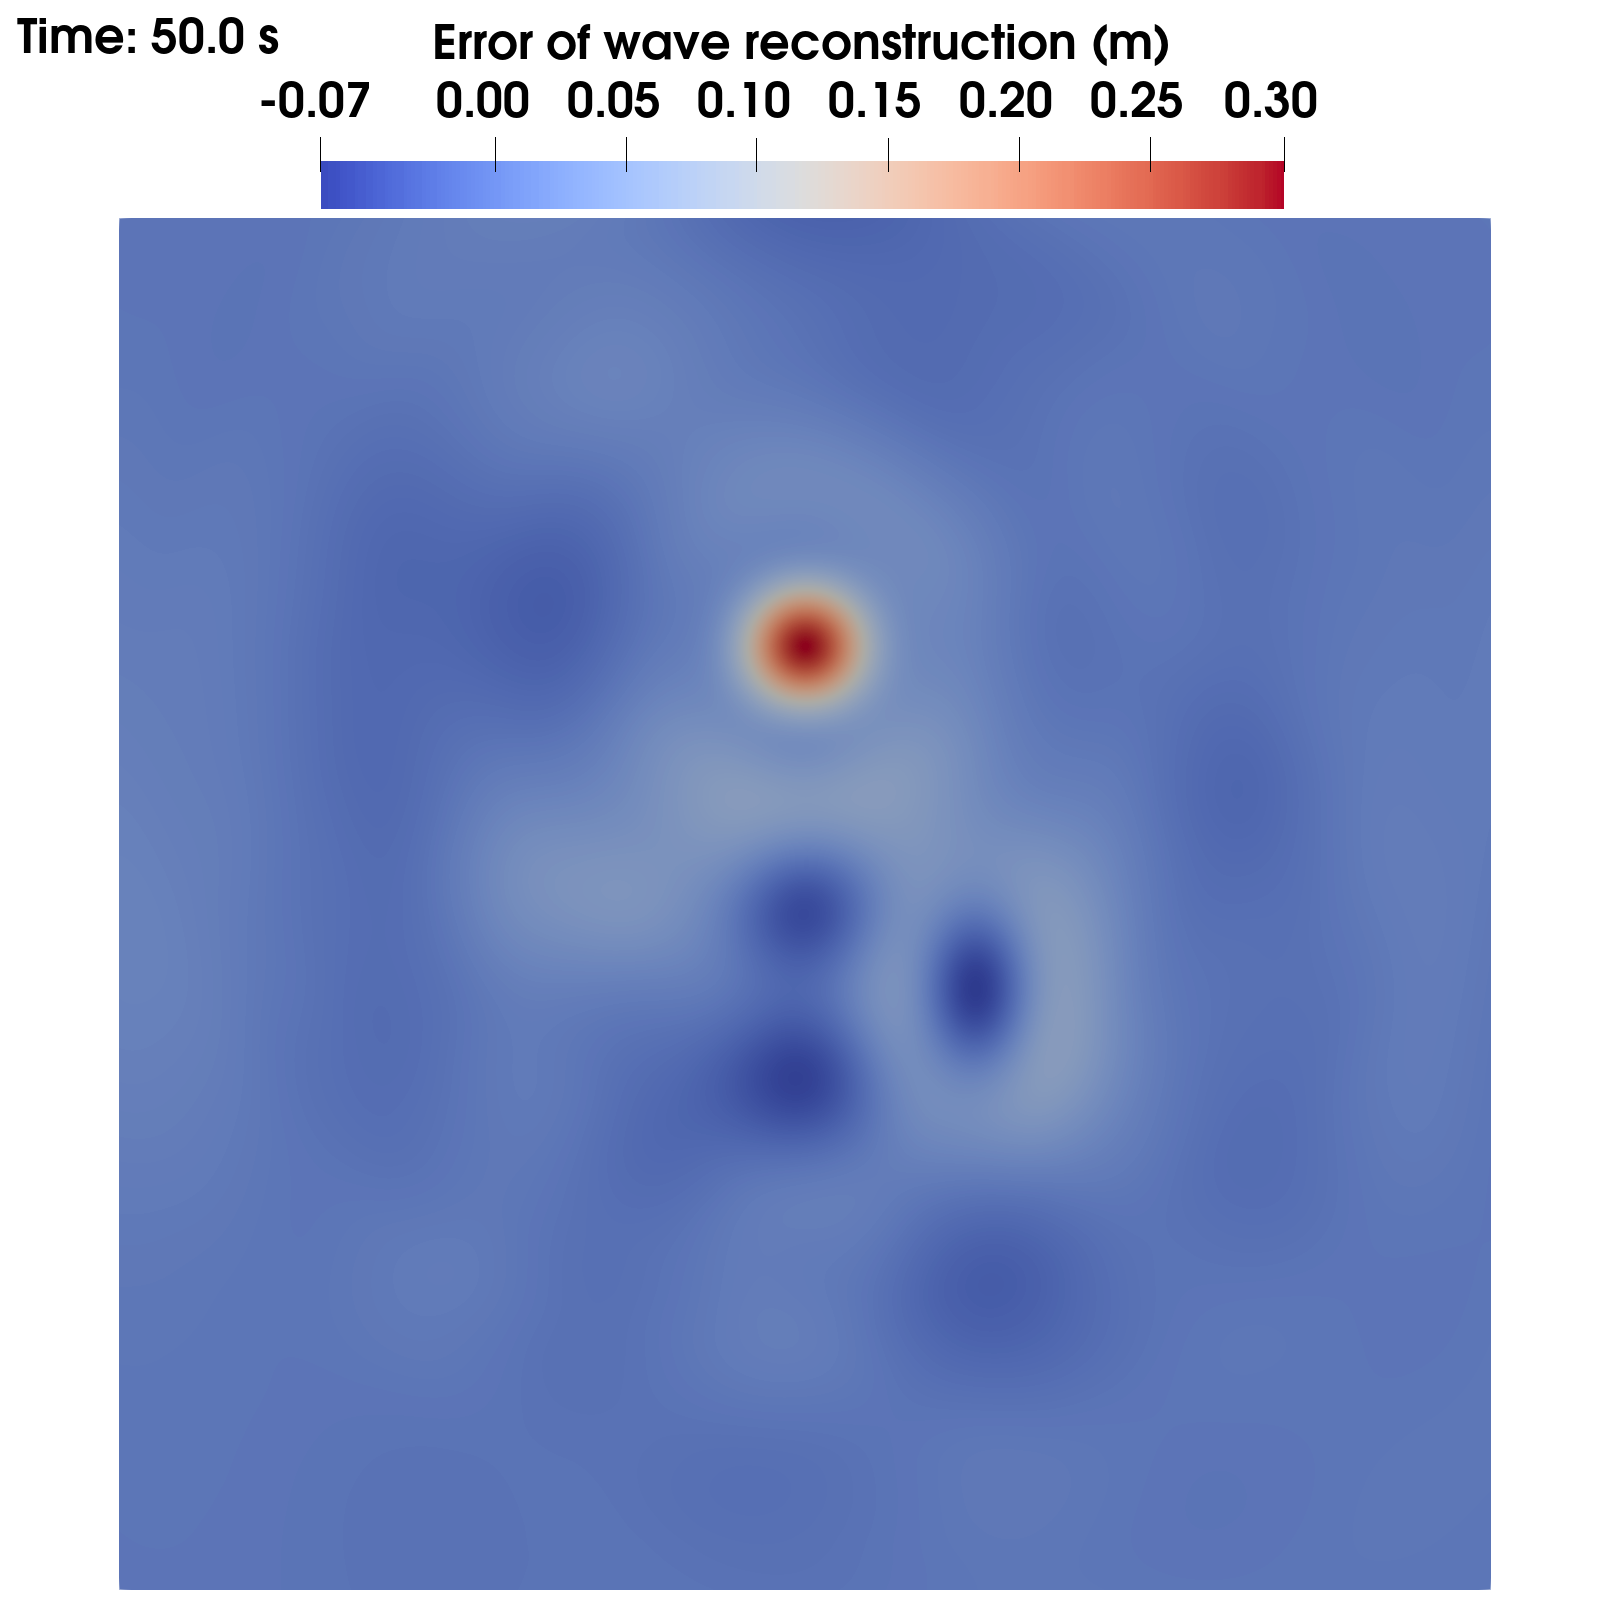
\includegraphics[width=0.3\textwidth]{JMM/images/results/wave_diff.png}
        }
    \end{figure}
\end{frame}

\begin{frame}
    \frametitle{QoI Predictions and Uncertainty}
    \begin{figure}
        \centering
        \subfloat[\textbf{Left:} Sensor and QoI locations]{
            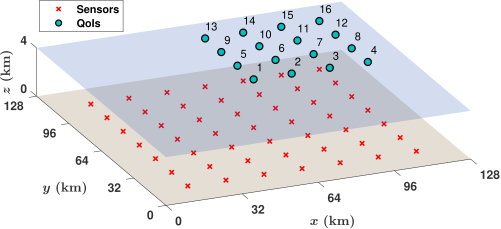
\includegraphics[width=0.45\textwidth]{JMM/images/test_config/sensor_qoi_locations.svg}
        }
        \hfill
        \subfloat[\textbf{Right:} QoI predictions and uncertainty for surface wave height]{
            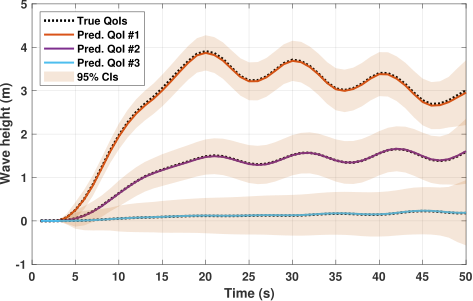
\includegraphics[width=0.45\textwidth]{JMM/images/results/qoi_vec_wave_height_uq_0_3.svg}
        }
    \end{figure}
    \begin{table}
        \toprule
        \textbf{Noise Level} & \textbf{Rel. Error} \\
        \midrule
        2\% & 0.0108 \\
        4\% & 0.0167 \\
        6\% & 0.0161 \\
        \bottomrule
    \end{table}
\end{frame}
